%  Article IJ 2008.tex (Version 1.0, 09/06/08)

%  The following commands have been added in the SPIE class
%  file (spie.cls) and will not be understood in other classes:
%  \supit{}, \authorinfo{}, \skiplinehalf, \keywords{}
%  The bibliography style file is called spiebib.bst,
%  which replaces the standard style unstr.bst.

\documentclass[]{spie}  %>>> use for US letter paper
%%\documentclass[a4paper]{spie}  %>>> use this instead for A4 paper

%% \renewcommand{\baselinestretch}{1.65}   %>>> 1.65 for double spacing, 1.25 for 1.5 spacing
%  The following command loads a graphics package to include images
%  in the document. It may be necessary to specify a DVI driver option,
%  e.g., [dvips], but that may be inappropriate for some LaTeX
%  installations.
\usepackage[]{graphicx, mdwlist}% mdwlist defines enumerate*, & itemize* to create COMPACT listings
\sloppy
\title{JACoP v2.0: improving the user experience with co-localization studies}
\author{Fabrice P. Cordeli\`{e}res\supit{a} and Susanne Bolte\supit{b}
\skiplinehalf
\supit{a}Institut Curie, CNRS UMR146, Plateforme d'Imagerie Cellulaire et Tissulaire, Orsay, France; \\
\supit{b}Institut des Sciences du V\'{e}g\'{e}tal, IFR87 ``La Plante et son Environnement", Plateforme d'Imagerie et de Biologie Cellulaire, Gif-sur-Yvette, France
}
\authorinfo{\\\supit{a}: E-mail: fabrice.cordelieres@curie.u-psud.fr, Telephone: +33 1 69 86 31 30\\  \supit{b}: E-mail: susanne.bolte@isv.cnrs-gif.fr, Telephone: +33 1 69 82 38 66}
%%>>>> when using amstex, you need to use @@ instead of @
%%%%%%%%%%%%%%%%%%%%%%%%%%%%%%%%%%%%%%%%%%%%%%%%%%%%%%%%%%%%%
%>>>> uncomment following for page numbers
% \pagestyle{plain}
%>>>> uncomment following to start page numbering at 301
%\setcounter{page}{301}
\begin{document}
\maketitle
%%%%%%%%%%%%%%%%%%%%%%%%%%%%%%%%%%%%%%%%%%%%%%%%%%%%%%%%%%%%%
\begin{abstract}
``Are my two proteins of interest at the same location?" Here is a question regularly asked... but rarely answered with precision. The cell biologist expects a yes-or-no answer. However, the use of imaging approaches implies that considering the current resolution, it can not be excluded that both proteins actually are at the same location. This statement is particularly emphasized when considering the evolutions of light microscopy. As an example, one might consider the recent work by Shroff \textit{et al.}\cite{HariShroff12182007} (see figure 4C and D) where PALM (PhotoActivated Localization Microscopy) has been used to overcome the diffraction limit encountered with regular microscopies such as wide field, confocal or TIRF microscopies. Their work proved that by pushing downward the resolution, originally co-localizing proteins appeared to be well apart. Co-localization studies must therefore always be considered relative to the resolution which has to be explicitly stated. \\
While setting the frame of reference is an easy step to go, the means to achieve co-localization studies are to date not so well known. This is mainly due to the widespread of generalist tools lacking information on their application domains and limits. In our previous work\cite{tutrev2006} we wanted to provide insight in current approaches to study co-localization and introduced two ImageJ plug-ins, JACoP (Just Another Co-localization Plug-in) and 3D object counter, those tools providing the user with means to test and use a wide range of methods. Since this field is highly controversial\cite{leted2007,ansleted2007}, we have now made an effort to explain alternative methodologies and simplifying JACoP to make it a more user friendly plug-in. In particular, its interface has been rethought and the plug-in is now totally macro recordable. In this communication we introduce the second version of JACoP and remind to the reader the field of application of methods, concluding with a decision tree.
\end{abstract}
%%%%%%%%%%%%%%%%%%%%%%%%%%%%%%%%%%%%%%%%%%%%%%%%%%%%%%%%%%%%
\keywords{Co-localization, ImageJ, image analysis, fluorescence microscopy.}
%%%%%%%%%%%%%%%%%%%%%%%%%%%%%%%%%%%%%%%%%%%%%%%%%%%%%%%%%%%%%
\section{INTRODUCTION}
\label{sec:intro} 
When working on co-localization, two major aims might be seeked. The first goal is to apply a co-localization method on a couple of images and to state if it exists and where it occurs. This might simply be done by overlaying both images, after an appropriate LUT has been attributed to each image. This first approach is a pre-requisite to the second, aiming for quantification of coincidence. Assessing the occurence of co-localization and identifying its spatial location will help restricting further analysis to the sometimes discrete sites of co-localization.
%%%%%%%%%%%%%%%%%%%%%%%%%%%%%%%%%%%%%%%%%%%%%%%%%%%%%%%%%%%%%
\section{METHODS AND RESULTS}
\label{sec:MM}
%%-----------------------------------------------------------
\subsection{What's new in JACoP ?}
\label{sec:New_JACoP}
\textbf{JACoP} has been totaly re-written, based on user feedback. The interface has been re-designed to offer full access to all the options, based on a unique Swing frame (see figure \ref{fig:interface}). It includes a ``Zoom/Reset button" which allows the user to set the two selected images side-by-side, automatically adapting the zoom. For each method selected, the user's attention is drawn on options to set, by highlighting the appropriate tab by turning its caption to red. 
\begin{figure}[!ht]
\begin{center}
\begin{tabular}{c}
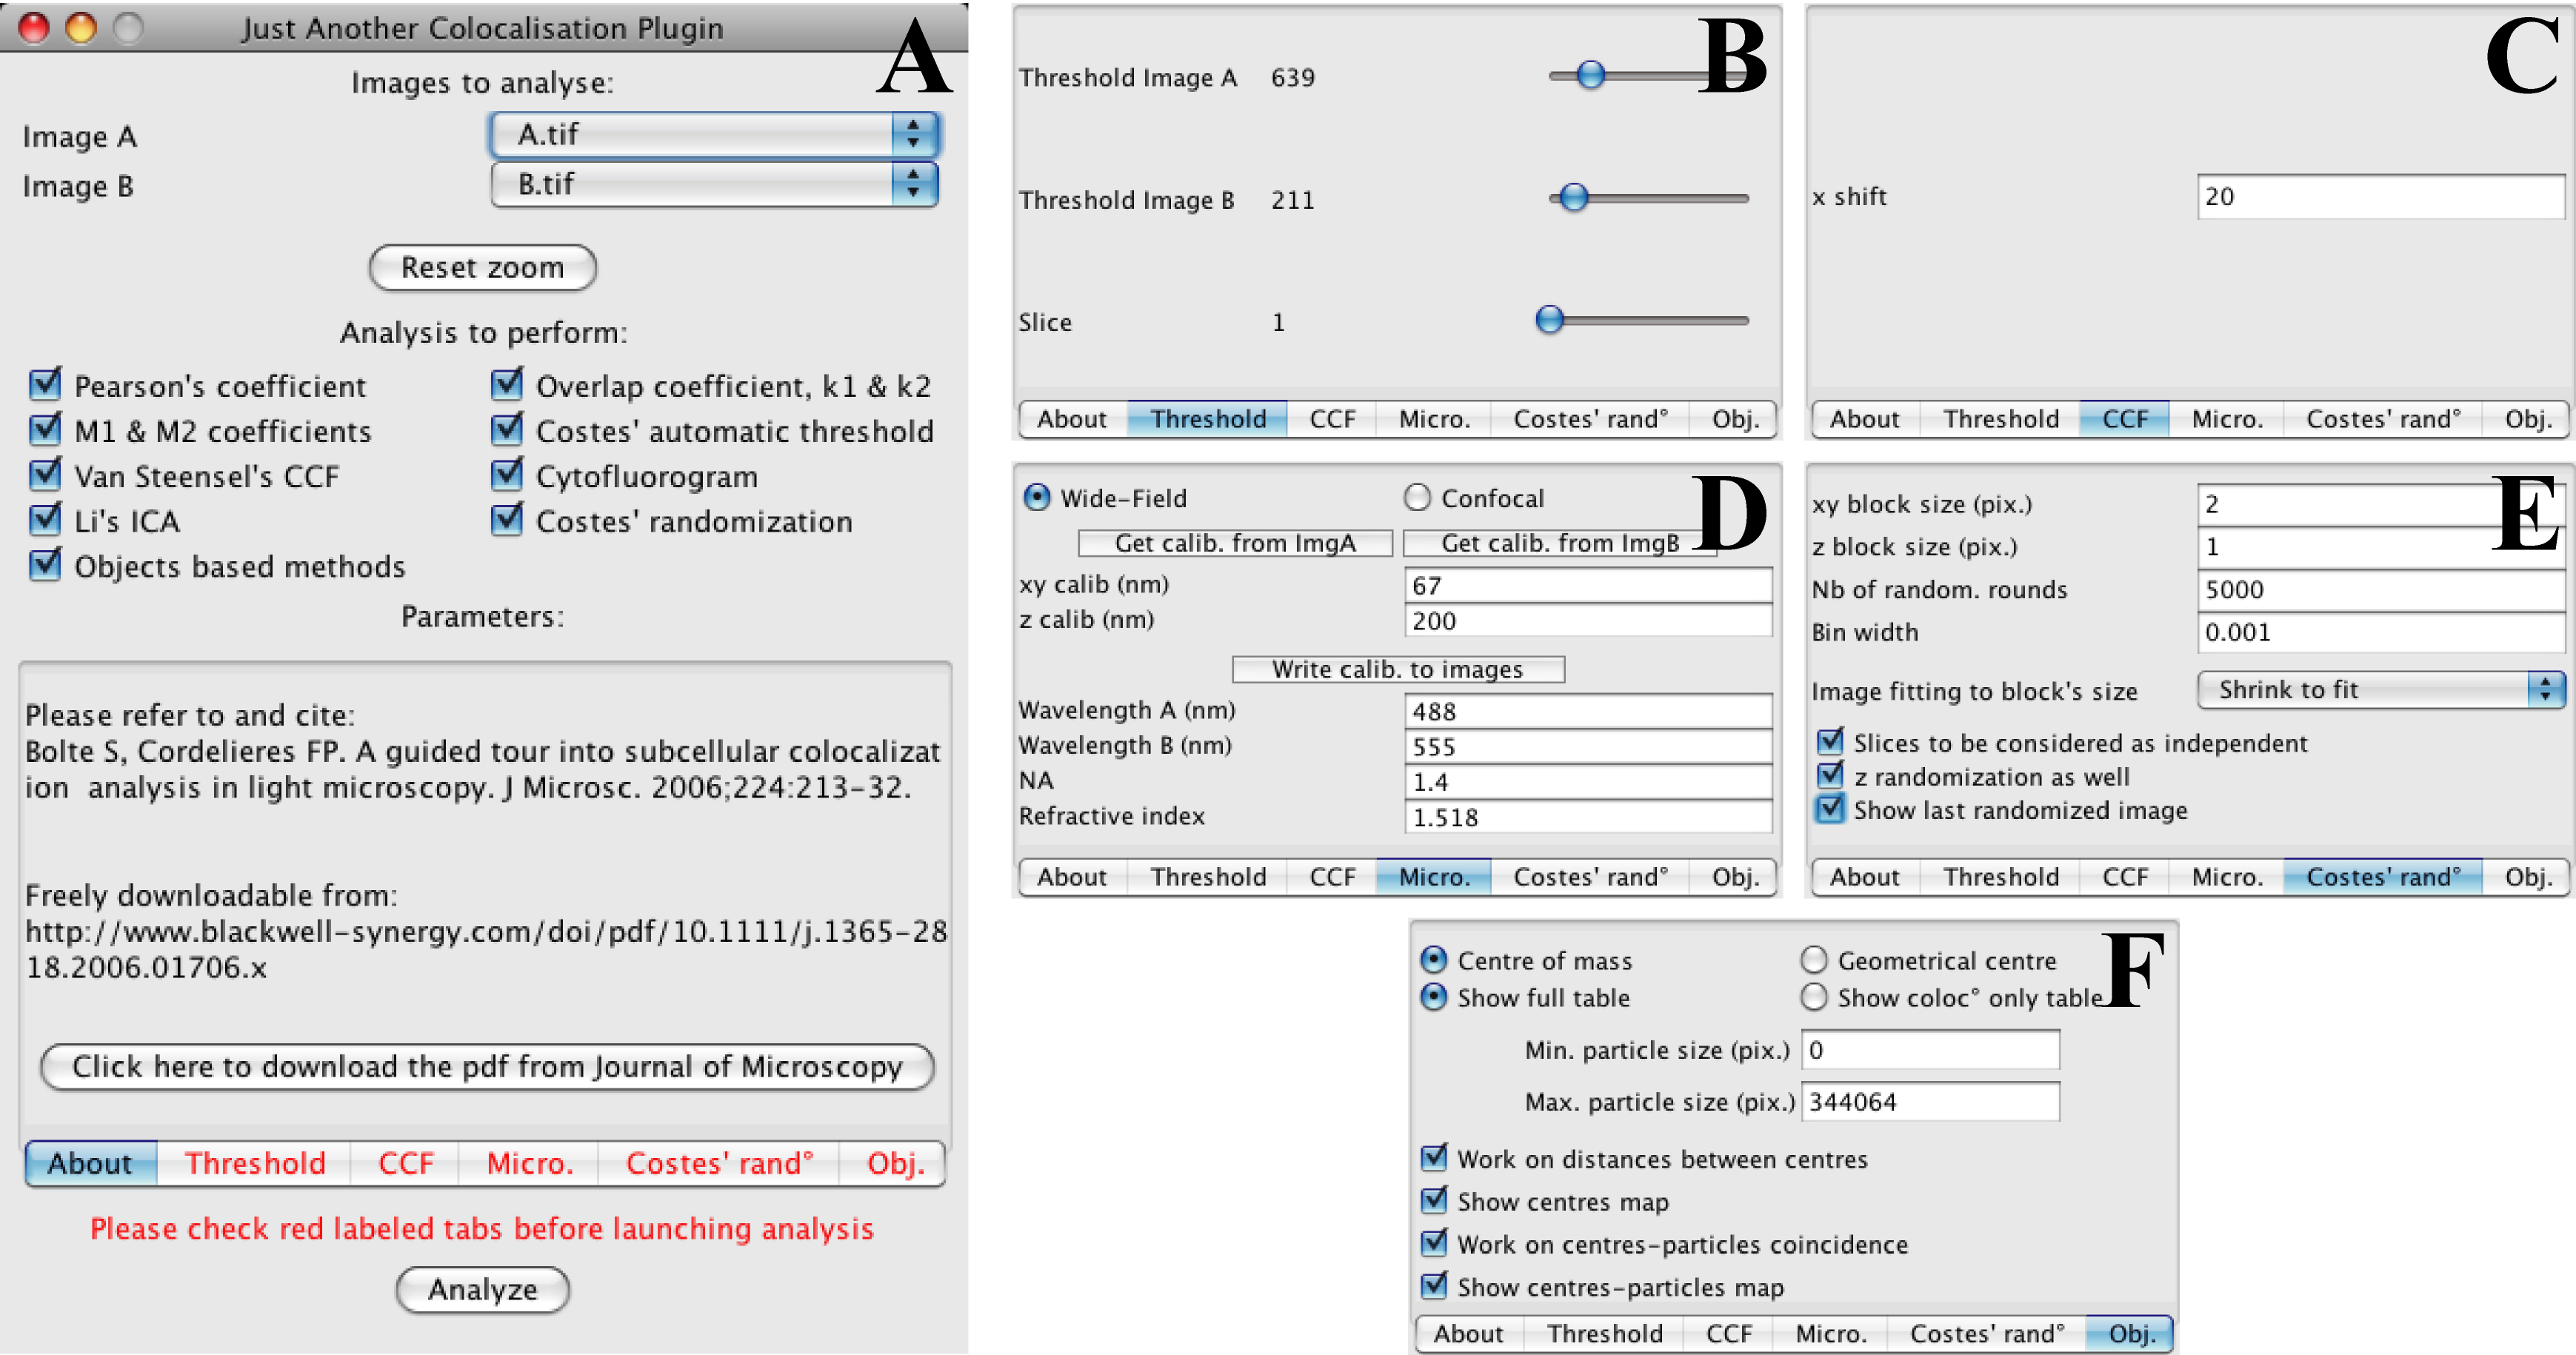
\includegraphics[width=0.9\linewidth]{figs/interface.png}
\end{tabular}
\end{center}
\caption[interface] 
%>>>> use \label inside caption to get Fig. number with \ref{}
{\label{fig:interface} 
Interface and options tabs of \textbf{JACoP}.}
\end{figure} 
%%-----------------------------------------------------------
\subsection{Cytofluorogram and Pearson's coefficient}
\label{sec:MM_cyto}
The most widely available method for co-localization estimation relies on plotting the \textbf{cytofluorogram}. In this representation, the intensities of channel A and B ($A_i$ and $B_i$ respectively, a and b being the channel's mean intensities) serve as coordinates for a dot on the graph. When a unique stoichiometry of association exists between the two proteins of interest, the dot cloud takes the shape of a line. The slope of the median line is related to the stoichiometry as well as characteristic parameters of the chromophores used for detection. Therefore, it can not strictly account for the ratio of association but might be used for comparison purposes between samples processed at the same time and in an identical fashion. The spread of the dot cloud relative to the median line might be estimated by the correlation coefficient, also called \textbf{Pearson's coefficient (PC)}\cite{Manders1992}.
\begin{equation}
\mbox{Pearson's coefficient:} \hspace{1cm} r_p=\frac{\sum_{i}(A_i-a)\times(B_i-b)}{\sqrt{\sum_{i}(A_i-a)^2\times\sum_i(B_i-b)^2}}
\label{eqn:Pearson}
\end{equation}
It must be emphasized that Pearson's coefficient is not a true quantification of co-localization but rather an estimate of the association strength between the two proteins considered. It varies from -1 to 1, -1 stating for inverse correlation (generally exclusion), 0 the absence of correlation and 1 a full correlation only achieved in biology when considering twice the same image. The difficulty generally begins when trying to set an absolute threshold between those three values. The question lies in mid-range values for which an absolute statement is hard to make. The workaround would be to have several experimental situations between which a comparison might be done. For instance, being able to increase/decrease the degree of association between the two proteins of interest would help setting the threshold. When only one experimental situation is available, other methods based on the Pearson's coefficient might be used (such as Costes' randomization). Three major pitfalls might arise when working with Pearson's coefficient:
\begin{enumerate*} % mdwlist defines enumerate*, & itemize* to create COMPACT listings
\item the stoechiometry of association is not unique: if possible, the workaround will be to restrict the analysis to a ROI of unique association rate;
\item poor signal to noise ratio: working on either or both, the sample preparation and image acquisition. Alternatively, methods have recently been proposed to try to isolate and/or take into account the noise compound from the image\cite{Adler2008};
\item bleedthrough from one channel to another or background: if not compromising too much the signal, both might be estimated and the coefficient calculated after use of an offset or threshold.
\end{enumerate*}
A variation of Pearson's coefficient, the \textbf{overlap coefficient}\cite{Manders1993}, might also be used. It is calculated by taking out average values from expression \ref{eqn:Pearson}:
\begin{equation}
\mbox{Overlap coefficient:} \hspace{1cm}r=\frac{\sum_{i}A_i\times B_i}{\sqrt{\sum_{i}A_i^2\times\sum_iB_i^2}}
\label{eqn:Overlap}
\end{equation}
As a result, the coefficient is always positive or null, ranging from 0 to 1, corresponding to no and full co-localization, respectively. The numerator has an important influence on the coefficient as each added product is equal to zero when one of the pixel value is background (i.e. equals to zero). As a consequence, this coefficient suffers from the same pitfalls as the Pearson's coefficient, especially when one or both images are corrupted by noise or background, giving raise to a non zero product. The same applies when comparing images with a discrete co-localisation. In this case, some particles might not have a counterpart in the other channel, letting the coefficient drop to zero. The overlap coefficient might therefore only be used in case the number of particles is equivalent between channels. When having a closer look at the way it is built, one might find the overlap coefficient being composed of two parts, the first depending on the amount of co-localised pixels intensities relative to the integrated squared intensities of channel A, the second being relative to the one of channel B. This way, the squared overlap coefficient could be expressed as a product of two new coefficients, \textbf{$k_1$} and \textbf{$k_2$}:
\begin{equation}
r^2=k_1\times k_2 \hspace{1cm} \mbox{with} \hspace{1cm} k_1=\frac{\sum_{i}A_i\times B_i}{\sum_{i}A_i^2} \hspace{1cm} \mbox{and} \hspace{1cm} k_2=\frac{\sum_{i}A_i\times B_i}{\sum_{i}B_i^2}
\label{eqn:k1k2}
\end{equation}
In case of perfect co-localization, meaning for each i $A_i=\alpha\times B_i$, $k_{1}$ will reach $\alpha$ and $k_{2}$ $\frac{1}{\alpha}$, where $\alpha$ is the slope of the mean line in the cytofluorogram (related but not equal to the proteins' stoechimetry). However, if one channel is corrupted by either noise or background, the denominator of the corresponding coefficient (here $k_1$ for channel A and $k_2$ for channel B) will increase and the coefficient itself drop. Looking at both coefficients is therefore usefull when the overlap coefficient is close to zero to identify the source of the problem. This is especially true when looking at the cytofluorogram has been unefficient on this matter. \\\\
All the previously described indicators may be calculated and the cytofluorogram drawn using \textbf{JACoP}: simply tick the appropriate tick boxes on the plug-in interface (``Pearson's coefficient", ``Overlapp coefficient, $k_1$ \& $k_2$" and ``Cytofluorogram", respectively). To proceed to analysis, click on the ``Analyze" button. A log window appears where each round of analysis starts with a dashed lined and the names of the images used as channel A and B. The calculated values are also available within this window. The cytofluorogram is drawn into a ``Plot window" and data might be exported to a tabler using the ``Save" button at the bottom of the window. Other methods for both intensity representation and co-localization assessment exist within \textbf{JACoP} such as \textbf{Li's method}. While the use of such method is simple within the plug-in (tick the ``Li's ICA" tick box), the reader is invited to refer to\cite{Li2004} and \cite{tutrev2006} for a more detailed description.
%%-----------------------------------------------------------
\subsection{Toward a first quantification of co-localization: Manders' coefficients \& Costes' automatic threshold}
\label{sec:MM_manders_CAThr}
While previous coefficients where rather suitable for comparative studies, no estimation of the amount of co-localization was reachable by their use. A step forward was made by making some modifications to the couple of $k$ coefficients proposed by Manders\cite{Manders1992}. The \textbf{$M_1$ and $M_2$ Manders' coefficient} are obtained as follows:
\begin{eqnarray}
Manders' coefficients: &M_1=\frac{\sum_{i}A_{i, coloc}}{\sum A_i} \hspace{0.5cm} with \hspace{0.5cm} A_{i, coloc}=A_i, if B_i>0 \\
&M_2=\frac{\sum_{i}B_{i, coloc}}{\sum B_i} \hspace{0.5cm} with \hspace{0.5cm} B_{i, coloc}=B_i, if A_i>0
\label{eqn:M1M2}
\end{eqnarray}
$M_1$ and $M_2$ are built by summing intensities of co-localizing pixels from one channel and dividing it by its integrated density. A pixel from channel A is considered as co-localized if it has a non zero intensity conterpart in the channel B. As a result, $M_1$ and $M_2$ give an estimate of the amount of co-localizing signal from a channel over another, without making any assumption on the stoechiometry it may adopt. This approach is therefore suitable when the amount of co-localization varies spatially. However, when at least one image is corrupted by noise, background or bleedthrough, the probability to find a non-null pixel in the second channel is increased: the coefficient is artificially reporting an increase of co-localization. Once more, appropriate sample preparation and acquisition is crucial. If the corruption source has an intensity signature well appart from the signal, one can try to use thresholding to calculate coefficients. This is achieved by working on the coefficients' definition: when calculating $M_1$, instead of considering $A_{i, coloc}=A_i$, if $B_i>0$, we can transform the condition into $B_i>thr_B$. The same assumption might be done for $M_2$. The question now remains on how to set $thr_A$ and $thr_B$. The commonly used method consist of asking the user for a visually estimated value. This method is highly suggestive and should be kept only when a set of image couples are processed. In this situation, both values should be determined on the most corrupted experimental situation and kept for the rest of the analysis.\\
An elegant way to determine thresholds has been proposed by Costes \textit{et al.}\cite{Costes2004}. On a cytofluorogram, the expected location of pixels representing noise is close to the origin, taking the shape of a formless cloud. When isolated, this population has a Pearson's coefficient of zero. The right couple of thresholds will therefore be reached when all pixels carrying intensities $(A_i, B_i)$ such as $A_i<thr_A$ and $B_i<thr_B$ have a Pearsons's coefficient equal or below zero. $thr_A$ is initially set to the maximum intensity of channel A, $thr_B$ is calculated based on the linear regression operated on the cytofluorogram's data. Then the correlation coefficient $r_p$ of pixels intensities below thresholds is estimated. While $r_p>0$ the previous process is applied, $thr_A$ being decremented by 1 at each iteration. This is the exact way this method is implemented within \textbf{JACoP}.\\
Avoiding user input is apparently a good approach. However , it finds its limits with poor signal-to-noise ratio images. In such a situation, the noise pixel's cloud encompass part of the signal pixels' cloud on the cytofluorogram. As a consequence, automatic thresholding will result in underestimating co-localisation. Moreover, the question of selecting threshold is more complex when considering a full dataset: should the thresholds be set once for all ? Based on which couple of images ? Should they be set automatically for each couple of images ? Of course, the most appropriate answer would be to work on image acquisition to acquire all image couples in the same way.\\\\
To calculate Manders' coefficient with \textbf{JACoP}, first tick the ``$M_1$ \& $M_2$ coefficients" box: the ``Threshold" tab turns to red. Two sliders allow setting both $thr_A$ and $thr_B$, the third slider allowing to navigate simultaneously on slices of the stack when working with 3D images (see figure \ref{fig:interface}B). Click on ``Analyze": the results are sent to the log window. The results takes form a two sets of information: coefficients calculated without and with thresholds ($thr_A$ and $thr_B$ are also logged). For Costes' automatic threshold retrieval, tick the appropriate box. No settings are required, so simply click ``Analyze" to start. The $thr_A$ and $thr_B$ values are available as well as $r_p$ values for pixels above and below thresholds and $M_1$ \& $M_2$ calculated with the retrieved thresholds. A plot window opens, carrying a representation of $r_p$ of pixels below thresholds as a function of $thr_A$. Finally, an image is created, presenting the co-localized pixels in white, other pixels appearing with their channel's LUT (green and red).
%%-----------------------------------------------------------
\subsection{Revisiting Pearson's coefficient use: Van Steensel's CCF \& Costes' randomization}
\label{sec:CCF_CRand}
Over the past ten years, major improvements have been made to overcome the limitations of the Pearson's coefficient. Two of those may help to use the coefficient in order to place a diagnostic on a couple of images or to provide a statistical degree of significance for the calculated value.\\
First, Van Steensel and colleagues\cite{VanSteensel1996} introduced the \textbf{cross-correlation coefficient (CCF)}. Basically, it consists of calculating the PC while operating a shift of one of the images relative to the other, then plotting the retrieved PC as a function of the displacement. In case of a true co-localization situation, the correlation will be lost while the displacement is done. As a consequence, the PC will decrease, reaching values close to zero when the structures from image A are outside the area/volume occupied by the ones from image B. On the graph, this situation is identified by a bell like shape. Its full width at half maximum (FWHM) depends on the relative sizes of structures. The difference between the maximum and the minimum height of the curve will obviously depend on the amount of co-localized signal, on the density of structures and the amount of noise corrupting both images. In the opposite situation, when signals are mutually exclusive, in the start situation (no shift) the PC is at its minimum. While shifting one image, the chance to get an overlap between structures from both channels increases, raising the PC value. The curve appears therefore as a hollow, with the same quantitative measurements as for the previous case being possible.\\
The CCF improves the co-localization diagnostic in two ways. First, it helps identifying two cases in quite a rapid fashion, by simply looking at the shape of the curve: true co-localization and exclusion. Second, by introducing several measures over a single couple of images, it helps overcoming the PC relative susceptibility to noise. In degraded signal-to-noise situations, the shape of the CCF will be unchanged, while the distance between its extrema will be reduced. This is mainly due to the co-occurence on the same location of noise from one channel and the signal from the other. CCF may therefore help assessing that the calculated PC actually reflects co-localization, even in cases where its value is away from its more easy to interpret boundaries.\\\\
To calculate the CCF using \textbf{JACoP}, first tick the ``Van Steensel's CCF" box. Go to the ``CCF" tab (see figure \ref{fig:interface}C): the ``$x_{shift}$" needs to be set, representing the maximum displacement, expressed in pixels, to be achieved in both directions. Click on ``Analyze": the results are sent to the log window, consisting of the CCF extrema (minimum and maximum values of PC) and the respective shifts for which they are achieved. Ideally, in case of co-localization, the maximum value is reached in the absence of displacement. If not, in most of the cases this is likely due to chromatic aberration which should be evaluated and corrected prior to any measurement. A plot window opens, carrying a representation of PC as a function of the ``$x_{shift}$".\\\\
Second, a step forward in the analysis based on PC might be reached by estimating the significance of the value by statistical means. The approach proposed by Costes \textit{et al.}\cite{Costes2004} relies on relocating the signal of one of the images in a randomized fashion, breaking the spatial co-occurence of signals, if any. Each couple of images obtained this way is a representation of co-localization events occurring by chance. By repeating the operation, a density distribution of PC probability is built, which represents a sample of the PC values that might be obtained while the only co-localization events occurring are due to hazard. The original PC is compared to this distribution to extract the probability of obtaining co-localization simply by chance.\\\\
To achieve the Costes' randomization in \textbf{JACoP}, first tick the ``Costes' randomization" box: the ``Micro" and ``Costes' rand$^\circ$" tabs turn to red. Go to the ``Micro" tab (see figure \ref{fig:interface}D): choose the appropriate microscope setup (confocal or wide-field), enter the xyz calibration values (i.e. pixels' size along each dimension) or retrieve from image A or B using the appropriate button and finally fill in information on the emission wavelengths, numerical aperture of the objective and refraction index of the immersion oil used. Go to the ``Costes' rand$^\circ$" tab (see figure \ref{fig:interface}E): values for xy and z blocks sizes have been calculated from values entered on the ``Micro" tab. To build the randomised images, pixel blocks are created which will be shuffled. In \textbf{JACoP}, randomization is achieved by first creating columns of pixels on the image which will be shifted either upward of downward by a number of rows which will be determined by drawing two random numbers (one for the direction, an other one for the displacement). This operation is repeated for each dimension of the image/stack to get the final randomised result. In case the Shannon/Nyquist sampling theorem has been followed during image acquisition, each resel (resolution element) will appear on at least 2 pixels, therefore creating a local intensity correlation on the image. To keep this correlation, pixels blocks of the corresponding size should be created. Number of rounds of randomization might then be set using the corresponding number field. The bin width is used to create the probability density histogram, the value stating for the width of each element on the representation. The pull-down menu ``Image fitting to the block's size" is used to control the behaviour of the plug-in in case the image's size is not a multiple of the block's size. ``Shrink to fit" is the more likely to be used, leaving aside the last few pixels in each dimension which would not fit entirely within a pixel block. The ``Pad with black pixels" option will increase the image size to fill the partially empty last pixel block. When the ``Slices to be considered as independent" option is ticked, different randomization in xy will be applied to each slice and z randomization will not be done (should be used only if the stack does not account for a 3D sample, but rather contains several independent fields of view). The two following tick boxes are used to randomize stacks (``z randomization as well" option) and ``Show last randomised image". Click on ``Analyze": the results are sent to the log window, consisting of the original PC, the range of the PCs retrieved after randomization, as well as the degree of significance of the original value (P-value). A plot window opens, carrying a representation of the probability to obtain each single PC range.\\
%%-----------------------------------------------------------
\subsection{Objects based analysis}
\label{sec:MM_OB}
There are two ways of taking into account the information carried by an image: it is both a collection of intensities that might be considered as independent, and a collection of objects. In the next part, we will see how \textbf{JACoP} might help co-localization evaluation, based on parameters retrieved from objects.\\
The first step will be to sort pixels into two categories, namely background and object, a step known as segmentation. Pixels constitutive of structures are then packed into objects based on their links with adjacent pixels (connexity analysis step). Once identified, descriptors might be calculated for each object, such as the coordinates of their centres (geometrical or of mass), their volume and surface etc... In the previous version of \textbf{JACoP}, this step was not implied directly and required an additional plug-in: 3D Object Counter. Now this has been improved and 3D Object Counter has been integrated within the second version of the plug-in.\\
Now that object analysis is possible, which ways do we have to measure co-localization ? In case of isotrope, rather uniformly labelled structures, Lachmanovich \textit{et al.}\cite{Lachmanovich2003} have proposed to simplify the image by making measurements only on the objects' centres. Considering a same object doubly labelled, both retrieved objects being of same size, the distance between their respective centres should be below the optical resolution. In case of inhomogeneous distribution of the signal, the centroid position will be influenced and therefore should be left appart to the benefit of the geometrical centre. Co-localization measurement is then expressed as the percentage of positive couples divided by the overall number of structures for the current channel. Due to the sampling frequency used when acquiring the image, signals might be co-localised while not appearing strictly at the same location ! As a single resel appears on at least two pixels in ideal situation, the overlap might be displaced by up to 2 pixels while still having to be considered as a true co-localization event. Therefore, measuring the distance might lead to a decrease in the false negative co-localizing objects. In this matter, the reference distance is quite easy to determine in 2D as it corresponds to the xy resolution: while considering the centre of the structure on image A, a structure of image B will be co-localized if it is present within a circle traced around centre A of a radius equal to the xy resolution. Due to the disparate resolutions over the three dimensions, this distance is not so easy to calculate in 3D. However, the answer might come from the observation of the factor limiting the resolution: the PSF (Point Spread Function) and more precisely the first Airy disc which might be approximated in 3D as having an ovoid shape (see figure \ref{fig:obj}A). Therefore in 3D, the reference distance is calculated by considering a reference point and fitting a 3D ellipse around it for which the two characteristic radii correspond to x/y and z resolutions. In this matter changing from Cartesian coordinates to Polar coordinates make it more easy to calculate the reference distance. In \textbf{JACoP} the two characteristic angles, the \textbf{azimuth $\Phi$} and the \textbf{zenith $\Theta$} (see expression \ref{phiTheta}) are first calculated, based on the coordinates of the two centres to analyse. Knowing this orientation, as well as the x, y and z resolutions ($resol^\circ_{x}$, $resol^\circ_{y}$ and $resol^\circ_{z}$ respectively), the distance from the reference centre to the border of the ovoid shape \textbf{$r_{ref}$} is calculated (see expression \ref{refDist}). The inter-centre distance \textbf{$r$} is then compared to this reference distance to assess if co-localization occurs (see figure \ref{fig:obj}C) or not (see figure \ref{fig:obj}B).
\begin{figure}[!ht]
\begin{center}
\begin{tabular}{c}
\includegraphics[width=0.75\linewidth]{figs/objFig.png}
\end{tabular}
\end{center}
\caption[obj] 
%>>>> use \label inside caption to get Fig. number with \ref{}
{\label{fig:obj}
Object based co-localization principle. (A) Centres of objects A and B are draw a a red and green sphere, respectively. The PSF is schematised in yellow, while the first Airy volume appears in orange. The former width, height and depth define the resolution along the 3 axis; (B) A and B are not co-localized as $r>r_{ref}$; (C) A and B are co-localized as $r\le r_{ref}$.}
\end{figure}
\begin{eqnarray}
\Phi=\arccos\frac{x_{B}-x_{A}}{\sqrt{(x_{B}-x_{A})^2+(y_{B}-y_{A})^2}} \hspace{0.5cm} \mbox{and} \hspace{0.5cm} \Theta=\arccos\frac{z_{B}-z_{A}}{\sqrt{(x_{B}-x_{A})^2+(y_{B}-y_{A})^2+(z_{B}-z_{A})^2}}\label{phiTheta}\\
r_{ref}=\sqrt{(resol^\circ_{x}\times\sin\Theta\times\cos\Phi )^2+(resol^\circ_{y}\times\sin\Theta\times\sin\Phi)^2+(resol^\circ_{z}\times\cos\Theta)^2\label{refDist}}
\label{eqn:objBased}
\end{eqnarray}
For objects having dimensions close to the optical resolution, an alternative method exists, which does not require those measurements. As the vast majority of such structures is located  precisely along this so called ovoid shape, the way to measure co-localization is even simplier to achieve: it consist in counting the number of centres from objects of image A falling inside segmented objects from image B.
Both methods are implemented within \textbf{JACoP}. To use one of them, tick the ``Objects based method" box. As a consequence, three tabs turn to red: ``Threshold" (should be set  to discriminate between background and object pixels), ``Micro." (enter here the acquisition parameters which will be used to determine the resolutions) and ``Obj.". Under this last tab (see figure \ref{fig:interface}F), a choice must me made on using either the ``Centre of mass" or ``Geometrical centres", depending on the spread of the signal, as previously pointed. Two reports might be obtained, taking form of a results table. The first, ``Show full table" will result in logging all information about all possible couples of centres and/or couples of centres-particles. The second option, ``Show coloc$^\circ$ only table" will only carry information on co-localizing couples, if any. A filter, based on particles sizes might be used, especially in case of images being corrupted by noise which might not have been excluded while thresholding the image (see parameters ``Min. particle size (pix.)" and ``Max. particle size (pix.)"). The choice of the type of analysis is made by ticking at least one of the two options ``Work on distance between centres" and/or ``Work on centres-particles coincidence". In the latter case, centres will be determined on centres from the image selected as ``Image A", while particles will be considered from ``Image B". In both methods, a recapitulative image might be built by ticking the appropriate box. ``Show centres map" will show as green dots non co-localizing centres from ``Image A", as red dots non co-localizing centres from ``Image B", as cyan dots co-localizing centres from ``Image A", as magenta dots co-localizing centres from ``Image B" and as yellow dots co-localizing centres from ``Image A" and ``Image B" perfectly appearing at the same location. ``Show centres-particles maps" will display centres from ``Image A" in green if not co-localizing (yellow otherwise), overlapping particles retrieved from ``Image B" (red). In case ``Show coloc$^\circ$ only table" is ticked, only co-localizing centres and/or particles will be displayed.
%%%%%%%%%%%%%%%%%%%%%%%%%%%%%%%%%%%%%%%%%%%%%%%%%%%%%%%%%%%%%
%\section{RESULTS}
%\label{sec:Results}
%%%%%%%%%%%%%%%%%%%%%%%%%%%%%%%%%%%%%%%%%%%%%%%%%%%%%%%%%%%%%
\section{CONCLUSIONS}
\label{sec:Conclusion}
\textbf{JACoP} has been improved to provide the user with a more ergonomic interface, in order to retrieve easily valuable co-localization information out of images. Now that a wide range of methods have been made available, which one should be used? We propose to first start by overlaying images, identify region of interest and restrict further analysis the most relevant locations (see figure \ref{fig:DecisionTree}). It is also a good starting point to decide if the analysis should be done based on objects (if structures are discrete and well identifiable) or on intensities (for rather diffuse labelling). In the former case, the size and distribution of the signal on particles should be considered to choose between the two proposed methods (work on centre to centre distance or on centre/particle coincidence). While working on intensities, two aims might be sought: either assess the occurrence of co-localization, or estimate the amount of co-localization. To achieve the first, a plethora of methods exits among which the choice should be done depending on the number of experimental conditions used. If comparisons are to be done between several experimental conditions, the usual toolbox can be used (PC, cytofluorogram, Li's method, overlap coefficient). Van Steensel's and Costes' randomization methods are rather to be used in situation where a statement is sought based on a single experimental condition. To achieve a quantification of the amount co-localization, the k coefficients (which could also be used to troubleshoot problems in the use of the overlap coefficient, see above) as well as Manders' coefficients can be calculated. For the latter, thresholds can be automatically calculated using Costes' method.
\begin{figure}[!ht]
\begin{center}
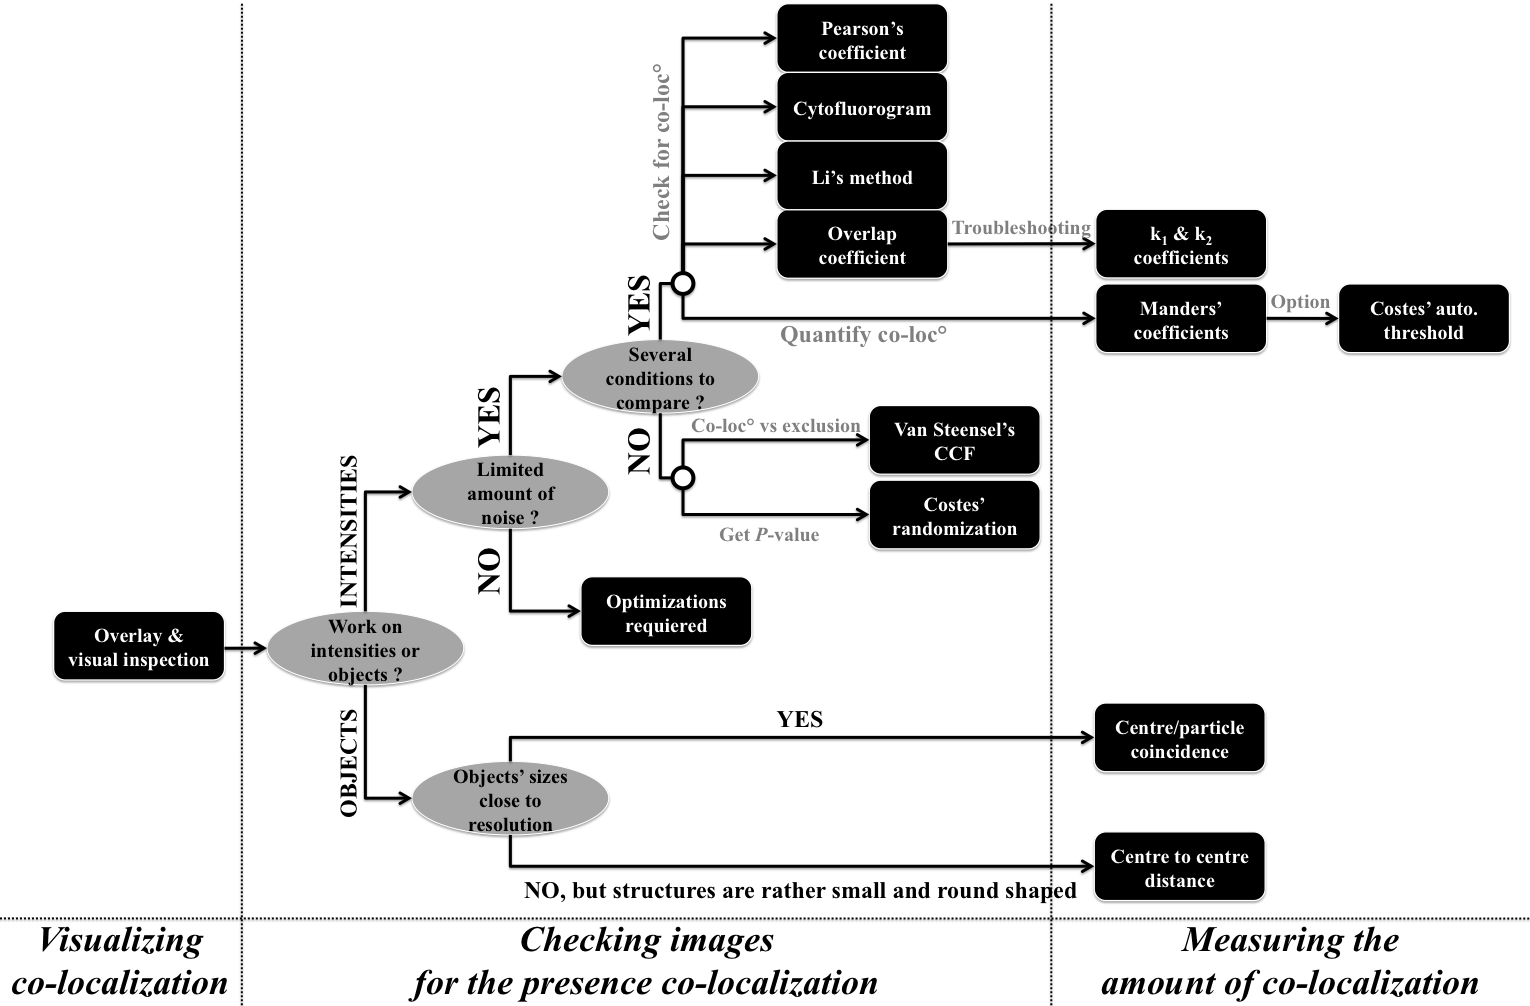
\includegraphics[width=0.85\linewidth]{figs/DecisionTree.png}
\end{center}
\caption[DecisionTree] 
{ \label{fig:DecisionTree} 
Proposed decision tree for choosing a co-localization method.}
 \end{figure} 
%%%%%%%%%%%%%%%%%%%%%%%%%%%%%%%%%%%%%%%%%%%%%%%%%%%%%%%%%%%%%
\acknowledgments     %>>>> equivalent to \section*{ACKNOWLEDGMENTS}
The authors would like to thank Thomas Boudier and Jim Dompierre for helpfull discussions, and the meeting organisers for giving us the opportunity to present the news features of \textbf{JACoP}.
%%%%%%%%%%%%%%%%%%%%%%%%%%%%%%%%%%%%%%%%%%%%%%%%%%%%%%%%%%%%%
%%%%% References %%%%%
\bibliography{JACoP}   %>>>> bibliography data in report.bib
\bibliographystyle{spiebib}   %>>>> makes bibtex use spiebib.bst
\end{document}
